\documentclass[11pt, spanish, a4paper, twoside]{article}

% Versión 1.er cuat 2021 Víctor Bettachini < vbettachini@unlam.edu.ar >

\usepackage[T1]{fontenc}
\usepackage[utf8]{inputenc}

% \usepackage[spanish, es-tabla]{babel}
\def\spanishoptions{argentina} % Was macht dass?
% \usepackage{babelbib}
% \selectbiblanguage{spanish}
% \addto\shorthandsspanish{\spanishdeactivate{~<>}}

\usepackage{graphicx}
\graphicspath{{./figuras/}{../LaTeX/}{../figurasLaTeX/}}
% \usepackage{float}

\usepackage[arrowdel]{physics}
\newcommand{\pvec}[1]{\vec{#1}\mkern2mu\vphantom{#1}}
% \usepackage{units}
\usepackage[separate-uncertainty= true, multi-part-units= single, range-units= single, range-phrase= {~a~}, locale= FR]{siunitx}
\usepackage{isotope} % $\isotope[A][Z]{X}\to\isotope[A-4][Z-2]{Y}+\isotope[4][2]{\alpha}

\usepackage{tasks}
\usepackage[inline]{enumitem}
% \usepackage{enumerate}

\usepackage{hyperref}

% \usepackage{amsmath}
% \usepackage{amstext}
% \usepackage{amssymb}

\usepackage{tikz}
\usepackage{tikz-3dplot}
\usepackage{tikz-dimline}
\usetikzlibrary{calc}
% \usetikzlibrary{math}
\usetikzlibrary{arrows.meta}
\usetikzlibrary{snakes}
\usetikzlibrary{decorations}
\usetikzlibrary{decorations.pathmorphing}
\usetikzlibrary{patterns}

\usepackage[hmargin=1cm,vmargin=3cm, top= 0.75cm,nohead]{geometry}

\usepackage{lastpage}
\usepackage{fancyhdr}
\pagestyle{fancyplain}
\fancyhf{}
\setlength\headheight{28.7pt} 
\fancyhead[LE, LO]{\textbf{Computational Analytical Mechanics} }
% \fancyhead[LE, LO]{\textbf{Mecánica General} }
\fancyhead[RE, RO]{\href{https://ingenieria.unlam.edu.ar/}{$\vcenter{\hbox{
\includegraphics[height=1cm]{../../../../figurasLaTeX/ambos.pdf}}}$}}  %edg fix path
\fancyfoot{\href{https://creativecommons.org/licenses/by-nc-sa/4.0/deed.es_ES}{$\vcenter{\hbox{
\includegraphics[height=0.4cm]{../../../../figurasLaTeX/by-nc-sa_80x15.pdf}}}$} \href{https://ingenieria.unlam.edu.ar/}{DIIT - UNLaM}}  %edg fix path
\fancyfoot[C]{ {\tiny Updated on \today} }
\fancyfoot[RO, LE]{Pág. \thepage/\pageref{LastPage}}
\renewcommand{\headrulewidth}{0pt}
\renewcommand{\footrulewidth}{0pt}


\begin{document}
\begin{center}
  % \textsc{\large Mecánica general}\\
  \textsc{\large Fuerzas externas en el enfoque Lagrangiano}
\end{center}

\begin{enumerate}

\item 
%\textbf{MIT Pset ? ex ?} 
\begin{minipage}[t][4.8cm]{0.55\textwidth}
\textbf{Barra que pende de un carro}\\
Obtenga las ecuaciones que describen la dinámica del sistema.
El momento de inercia para una barra de masa \(m\) y longitud \(l\) para una rotación desde uno de sus extremos es \(\frac{m}{12} l^2\). 
\begin{enumerate}
	\item Calcule el Lagrangiano.
	\item Descomponga en fuerzas generalizadas las no conservativas que actúan sobre el sistema:
	\begin{itemize}
		\item el forzado externo \(\vec{F}(t)\),
		\item y la que hace ejerce amortiguador de constante \(b\) en función de la velocidad del carro,  \(- b \dot{x} \hat{x}\).
	\end{itemize}
	\item Calcule las ecuaciones de Euler-Lagrange. 
\end{enumerate}
\end{minipage}
\begin{minipage}[c][0cm][t]{0.4\textwidth}
	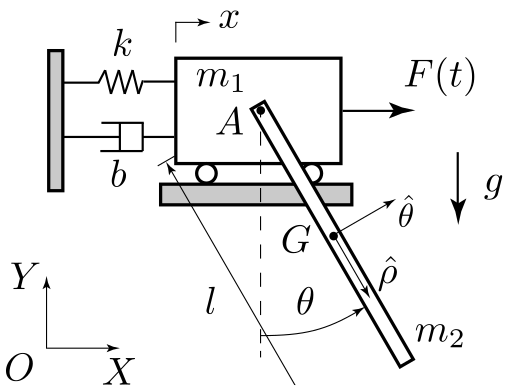
\includegraphics[width=\textwidth]{zweite}
\end{minipage}




\item 
%\textbf{MIT Pset 7 ex 2} 
\begin{minipage}[t][5.5cm]{0.6\textwidth}
\textbf{Péndulo de torsión desbalanceado}\\
Dos pesos de masa idéntica $m$ están unidos al extremo de brazos de masa despreciable.
Uno de los brazos describe una inclinación fija con la horizontal de $\phi$.
Descartamos la fricción con los rodamientos que mantiene vertical el eje de donde parten los brazos.
Este puede rotar libremente a cualquier ángulo $\theta$ pues un resorte de torsión de constante elástica $K_t$ opone un torque cada vez que $\theta \neq 0$.
En adición a este torque se ejerce uno externo variable en el tiempo: $\vec{\tau}= \tau (t) \hat{z}$.

Pregunta conceptual:
¿Cuales es la unidad de la fuerza generalizada?
\begin{tasks}(5)
	\task \si{\newton}
	\task \si{\newton \over \metre}
	\task \si{\newton \metre}
	\task Otra
\end{tasks}
Despeje la aceleración angular de la ecuación para la dinámica de Euler-Lagrange. Resultado:
\[
	\ddot{\theta} = \frac{K_{T} \theta + \tau}{L^{2} m \left(\sin^{2}{\left(\phi \right)} - 2\right)}
\] 
\end{minipage}
\begin{minipage}[c][1cm][t]{0.35\textwidth}
	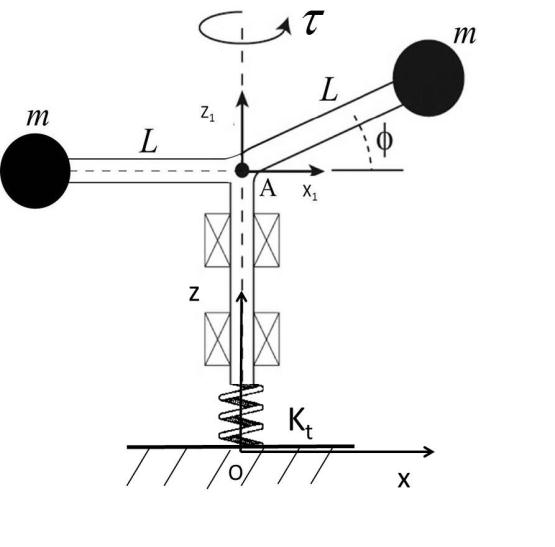
\includegraphics[width=\textwidth]{pset7ex2}
\end{minipage}



\item
%\textbf{MIT Pset 7 ex 4} 
\begin{minipage}[t][8cm]{0.6\textwidth}
\textbf{Barriles soldados}\\
Dos barriles cilíndricos homogéneos de respectivas masas y radios $m_1$,$m_2$, $R_1$ y $R_2$ están soldados.
Este armado rota sin fricción en torno a un eje.
Una cuerda de masa despreciable envuelve al cilindro externo y sus extremos conectan un resorte de constante elástica $k$ y un amortiguador.
Tal amortiguador ejerce una fuerza de resistencia al movimiento lineal con la velocidad,
$$
\vec{F}_\mathrm{amortiguador} = - b \dot{\vec{r}}.
$$

Una correa de masa despreciable envuelve al cilindro de menor radio y de ella pende vertical un bloque de masa $m_o$.\\
Despeje la aceleración angular de la ecuación de la dinámica de Euler-Lagrange. 
Resultado:\\
\[
	\ddot{\theta} = \frac{2 \left(R_{1} g m_{0} - R_{2}^{2} b \dot{\theta} - R_{2}^{2} k \theta\right)}{2 R_{1}^{2} m_{0} + R_{1}^{2} m_{1} + R_{2}^{2} m_{2}}
\]
\end{minipage}
\begin{minipage}[c][0cm][t]{0.35\textwidth}
	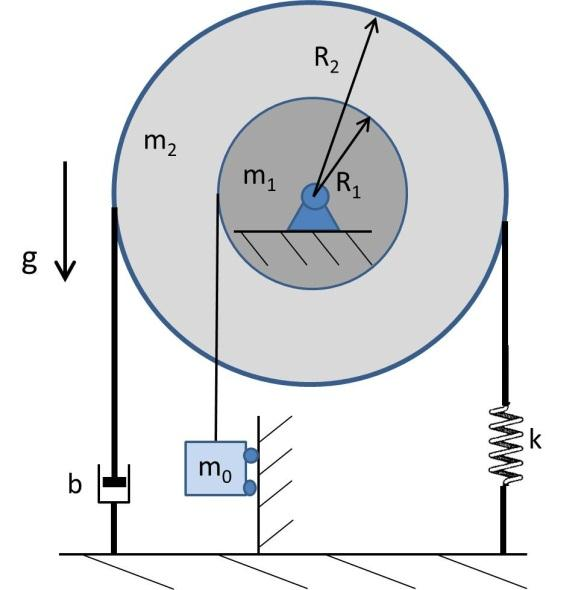
\includegraphics[width=\textwidth]{pset7ex4}
\end{minipage}



\item
%\textbf{MIT Pset 7 ex 6} 
\begin{minipage}[t][6cm]{0.5\textwidth}
\textbf{Plano inclinado oscilante}\\
Sobre la superficie inclinada en $\theta_0$ del carro de masa $m_0$ rueda sin deslizar un disco de radio $R$ y masa $m$.
Este no se sale de la superficie a pesar de que al centro del mismo se aplica una fuerza $\vec{F}= F(t) \hat{x}$ gracias a un resorte de constante elástica $K_1$ que une este centro con el carro.
Limita el alcance de este un resorte de constante elástica $K_2$ fijado a la pared y un amortiguador proporcional a la velocidad de constante proporcional $b$.
Ambos resortes tienen originalmente su longitud de equilibrio $l_{10}$ y $l_{20}$.
Se descarta la fricción del carro con el suelo.
Todo el sistema está sometido a la aceleración gravitatoria $\vec{g}= - g \hat{y}$.\\
\end{minipage}
\begin{minipage}[c][0cm][t]{0.45\textwidth}
	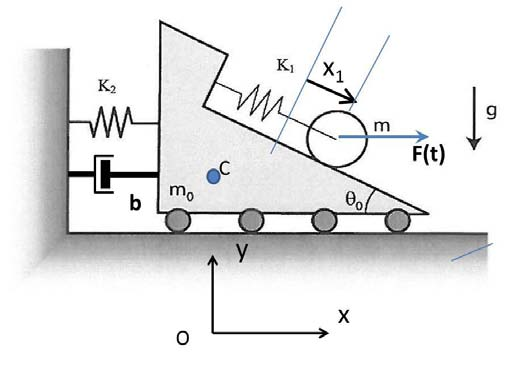
\includegraphics[width=\textwidth]{pset7ex6}
\end{minipage}
Pregunta conceptual: ¿Qué es la fuerza generalizada asociada al desplazamiento virtual $\delta x$ debida a $\vec{F}$?\\
\begin{tasks}(4)
	\task $F(t) \cos(\theta)$
	\task $F(t)$
	\task $F(t) \delta x$
	\task $0$
\end{tasks}
Obtenga las ecuaciones de la dinámica de Euler-Lagrange. 



\end{enumerate}
\end{document}
